\usepackage[utf8]{inputenc}
\usepackage[T1]{fontenc}
\usepackage{mathptmx}
\usepackage[scaled=.90]{helvet}
\usepackage{courier}
\usepackage{caption}
\captionsetup{labelformat=empty,labelsep=none}
\usepackage{verbatim}
\usepackage{hyperref}
\usepackage{listings}
% strikethrough (\sout)
\usepackage{ulem}
\lstset{language=Perl,basicstyle=\normalsize,tabsize=3,showstringspaces=false}

\title{Dancer and DBIx::Class}
\author[racke]{Stefan Hornburg (Racke)\\ \texttt{racke@linuxia.de}}
\date{Czech Perl Workshop, Prague, 21st May 2014}

\begin{document}
\maketitle{}

\begin{frame}
  \titlepage
\end{frame}

\tableofcontents

% \section{Übersicht}

% DBIx::Class ist mit Sicherheit einer der größten Schätze von "Modern Perl"
% und bietet schnelle und komfortable Datenbankabfragen.

% Ebenso erleichtert Dancer das Erstellen von Webanwendungen mit einer leicht
% verständlichen Programmierung.

% Wie können beide zusammen genutzt werden? Zunächst mit dem DBIC Plugin für
% Dancer. Mit diesem können mehrere DBIx::Class Schemas innerhalb der
% Dancer-Anwendung verwenden werden.

% Um auch die Dancer-Sessions in der Datenbank zu speichern, habe ich eine Engine für Dancer und DBIC geschrieben.

% Außerdem werde ich ein Projekt vorstellen, mit dem man einfach den Inhalt
% von Datenbanken mittels eines DBIx::Class Schemas editieren kann.

% \begin{frame}<handout:0>{Übersicht}
% \begin{itemize}
% \item Einführung
% \item DBIC Schemas mit Dancer Plugin
% \item DBIC session engine
% \item TableEditor
% \end{itemize}
% \end{frame}

% Wir starten mit einer kurzen Einführung von DBIx::Class.

\section{Introduction}
% \begin{frame}{Datenbank}
% \begin{itemize}
% \item Datenbank
% \item Tabellen
% \item Datensätze
% \end{itemize}
% \end{frame}

% \begin{frame}{DBIx::Class}
% \begin{itemize}
% \item Schema
% \item ResultSet
% \item Row / Objekt
% \end{itemize}
% \end{frame}

\subsection{Dancer}

Let's dance. I'm Racke from Hannover.pm in Germany and work
as self employeed programmer and system administrator.

My presentation today is about Dancer and DBIX::Class and how to use
them together.

Dancer is a micro web framework which makes it really easy
to write your own web application. Really so easy that it even
programmers from other languages like PHP and Ruby start with Perl
just because of Dancer.

Many web applications are using a relational database like MySQL
or Postgres. DBIx::Class is an Object Relational Mapper that provides
you with objects instead of just data. This is easier, more convenient 
and even faster to read and manipulate your database records.

So, let's start to dance first.
 
\begin{frame}{Easy to start with}
\begin{itemize}
\item Application ready to go
\item Syntax easy to understand
\item Routes and Keywords
\end{itemize}
\end{frame}

\begin{frame}[fragile]{Easy to start with}
\begin{itemize}
\item cpanm Dancer YAML
\item dancer -a Dropbox
\item cd Dropbox
\item ./bin/app.pl
\end{itemize}
\end{frame}
\begin{frame}[fragile]{Program}

\verb|./bin/app.pl|

\begin{lstlisting}

#!/usr/bin/env perl
use Dancer;
use Dropbox;
dance;

\end{lstlisting}

\end{frame}

\begin{frame}[fragile]{Module}

\verb|lib/Dropbox.pm|

\begin{lstlisting}

package Dropbox;
use Dancer ':syntax';

our $VERSION = '0.1';

get '/' => sub {
    template 'index';
};

true;
\end{lstlisting}
\end{frame}

\subsubsection{Templates}

The content will be rendered first and passed to the
layout renderer, so before\_layout\_render could mangle
with it.

The values passed to the template keyword are used
for both layout and content.

\begin{frame}{Templates}
\begin{figure}
\includegraphics[page=1,width=.6\textwidth]{layout.pdf}
\end{figure}
\end{frame}{Templates}

\begin{frame}[fragile]{Templates}
\begin{itemize}
\item Normal Layout
\begin{lstlisting}
template 'index', {name => 'Test'}
\end{lstlisting}
\item Specific Layout
\begin{lstlisting}
template 'index', {name => 'Test'}, {layout => 'test'}
\end{lstlisting}
\item No Layout
\begin{lstlisting}
template 'index', {name => 'Test'}, {layout => undef}
\end{lstlisting}
\end{itemize}
\end{frame}

\subsubsection{Routes}

Für eine Route benötigen wir

\begin{itemize}
\item HTTP-Methode
\item Pfad
\item Subroutine
\end{itemize}

\begin{frame}{Routes and Keywords}
\begin{itemize}
\item HTTP method
\begin{itemize}
\item get
\item post
\item ...
\item any
\end{itemize}
\item Path
\item Subroutine
\end{itemize}
\end{frame}

Der Pfad für eine Route kann in einer der folgenden
Weisen angegeben werden.

\begin{frame}{Routes}
\begin{itemize}
\item String
\item Named parameters
\item Wildcards 
\begin{itemize}
\item Splat
\item Megasplat
\end{itemize}
\item Regular expression
\end{itemize}
\end{frame}

\subsubsection{String}
\begin{frame}[fragile]{String}
\begin{lstlisting}
get '/home' => sub {
    my $files = autoindex('/');

    template 'filebrowser', {directory => 'Home',
                             files => $files,
                            };
};
\end{lstlisting}
\end{frame}

\subsubsection{Named parameters}
\begin{frame}[fragile]{Named parameters}
\begin{lstlisting}
get '/home/:file' => sub {
    my $files = autoindex(param('file'));

    template 'filebrowser', {directory => param('file'),
                             files => $files,
                            };
};
\end{lstlisting}
\end{frame}

\subsubsection{Splat}
\begin{frame}[fragile]{Splat}
\begin{lstlisting}
get '/images/covers/*.jpg' => sub {
    my ($isbn) = splat;

    if (-f "public/images/covers/$isbn.jpg") {
        return send_file "images/covers/$isbn.jpg";
    }

    status 'not_found';
    forward 404;
}
\end{lstlisting}
\end{frame}

\subsubsection{Megasplat}
Die einfache Wildcard matcht nur auf einen Teil des Pfads,
d.h. bis zum nächsten Schrägstrich (Slash).

Mit der doppelten Wildcard (Megasplat) wird einfach der 
Rest des Pfades gematcht und die \verb|splat|-Funktion
gibt eine Liste zurück.

\begin{frame}[fragile]{Megasplat}
\begin{lstlisting}
https://eshop.state.gov/lostpwd/biz@linuxia.de/e642bd543b9907bd2c06aa485261cb1a849a9f23fc7324bff45ebd35f4efe2cb

get '/lostpwd/**' => sub {
    my ($email, $hash) = splat;

    form->fill(email => $email,
               hash => $hash);
    
    template('lostpwd_confirm', form => $form);
}
\end{lstlisting}
\end{frame}

\subsubsection{Regular Expression}

\begin{frame}[fragile]{Regular Expression}

Catch-All (last route!)

\begin{lstlisting}
any qr{.*} => sub {
    ...
};
\end{lstlisting}
\end{frame}

\subsubsection{Keywords}
\begin{frame}[fragile]{Keywords}
\begin{itemize}
\item get, post, any, put, del, ...
\item request, params, param
\item redirect, forward, status, header
\item config, var, session
\item from\_json, to\_json, from\_xml, to\_xml
\end{itemize}
\end{frame}

\subsubsection{var(s) and session}
\begin{frame}[fragile]{var(s) and session}

Storing and retrieving data for the current request:

\begin{lstlisting}
var bar => 'pivo';
$bar = var 'bar';
$bar = vars->{bar};
\end{lstlisting}

Storing and retrieving data from the session:

\begin{lstlisting}
session username => 'racke@linuxia.de';

if (! session('username')) {
    redirect uri_for('/login');
}
\end{lstlisting}

\end{frame}

\begin{frame}{Easy to expand}
\begin{itemize}
\item Plugins
\item Hooks
\item Engines
\end{itemize}
\end{frame}

\begin{frame}[fragile]{before Hook}
Password protected site:
\begin{lstlisting}
hook 'before' => sub {
    unless (session('user')
        || request->path eq '/login'
        || request->path =~ m%^/lostpwd%
        ) {
        redirect '/login';
    }
};
\end{lstlisting}
\end{frame}

\begin{frame}{Solid}
\begin{itemize}
\item Stable
\item Keep behaviour
\item Community
\end{itemize}
\end{frame}

\begin{frame}{Applications}
\begin{itemize}
\item Simple Dropbox 
\url{https://metacpan.org/pod/Dancer::Plugin::Dropbox}
\item .state.gov Websites \\
\url{https://eshop.state.gov/}
\item Monitor for Power Plant
\end{itemize}
\end{frame}

\subsection{DBIx::Class}
\begin{frame}{DBIx::Class}
\begin{itemize}
\item ORM
\item Objects instead of SQL
\item Performance
\end{itemize}
\end{frame}

It took some time to get involved with DBIx::Class for various reasons.

\begin{frame}{DBIx::Class}
\begin{itemize}
\item Database => Schema
\item interchange6 => Interchange6::Schema
\end{itemize}
\begin{itemize}
\item Table => Result classes
\item users => Interchange6::Schema::Result::User
\end{itemize}
\begin{itemize}
\item Queries => Result sets
\end{itemize}
\end{frame}

\begin{frame}{User and Roles}
\begin{description}
\item[User]
\begin{itemize}
\item racke@linuxia.de
\item info@nite.si
\item test@linuxia.at
\end{itemize}
\item[Role]
\begin{itemize}
\item user
\item editor
\item admin
\item guest
\end{itemize}
\end{description}
\end{frame}

\begin{frame}{Tables}
\begin{itemize}
\item users
\begin{itemize}
\item users\_id
\item email
\item first\_name
\item ...
\end{itemize}
\item roles
\begin{itemize}
\item roles\_id
\item name
\item label
\end{itemize}
\item user\_roles
\begin{itemize}
\item users\_id
\item roles\_id
\end{itemize}
\end{itemize}
\end{frame}

\begin{frame}[fragile]{Roles for an user}
\begin{lstlisting}
mysql> select R.name from users U
       join user_roles UR on (U.users_id = UR.users_id)
       join roles R on (UR.roles_id = R.roles_id)
       where U.email = 'racke@linuxia.de';

+--------+
| name   |
+--------+
| user   |
| editor |
+--------+
\end{lstlisting}
\end{frame}

\begin{frame}[fragile]{User with DBIx::Class}
\begin{lstlisting}
$rs = $schema->resultset('User');
$user = $rs->find(1);
$user = $rs->find({email => 'racke@linuxia.de'});

$first_name = $user->first_name;

$users_linuxia = $rs->search({
    email => {like => '%@linuxia.de'}});
\end{lstlisting}
\end{frame}

\begin{frame}[fragile]{Roles with DBIx::Class}
\begin{lstlisting}
$rs = $schema->resultset('User');
$user = $rs->find({email => 'racke@linuxia.de'});

$roles = $user->roles;
\end{lstlisting}
\end{frame}

\begin{frame}[fragile]{User Result Class}
\begin{lstlisting}
package Interchange6::Schema::Result::User;

__PACKAGE__->table("users");

__PACKAGE__->add_columns(...);

__PACKAGE__->set_primary_key("users_id");

\end{lstlisting}
\end{frame}


\begin{frame}[fragile]{User Result Class}
\begin{lstlisting}
package Interchange6::Schema::Result::User;

__PACKAGE__->has_many("UserRole",
  "Interchange6::Schema::Result::UserRole",
  { "foreign.users_id" => "self.users_id" },
);

__PACKAGE__->many_to_many("roles", "UserRole", "Role");
\end{lstlisting}
\end{frame}

\subsubsection{Tips and Tricks}

\begin{frame}[fragile]{Object inflation}
\begin{lstlisting}
debug "Role: ", $role;

debug "Role: ", {$role->get_inflated_columns};
\end{lstlisting}
\begin{lstlisting}
Role: {'label' => 'User',
       'name' => 'user',
       'roles_id' => '3'} 
\end{lstlisting}
\end{frame}

\begin{frame}{Object vs Hashref}
\begin{itemize}
\item Debug / Logs
\item Templates
\item API / JSON
\item Speed
\end{itemize}
\end{frame}


\subsection{Database Administration}
\begin{frame}{Database Administration}
\begin{itemize}
\item \sout{phpmyadmin}
\item \sout{phppgadmin}
\item TableEditor
\end{itemize}
\end{frame}

\begin{frame}{TableEditor Features}
\begin{itemize}
\item Different database systems \\
      MySQL, PostgreSQL, ...
\item higher level of abstraction
\item modern frontend
\item concise source code
\item ``simple'' installation
\end{itemize}
\end{frame}

\begin{frame}[plain]{Input Database Parameters}
  \begin{center}
    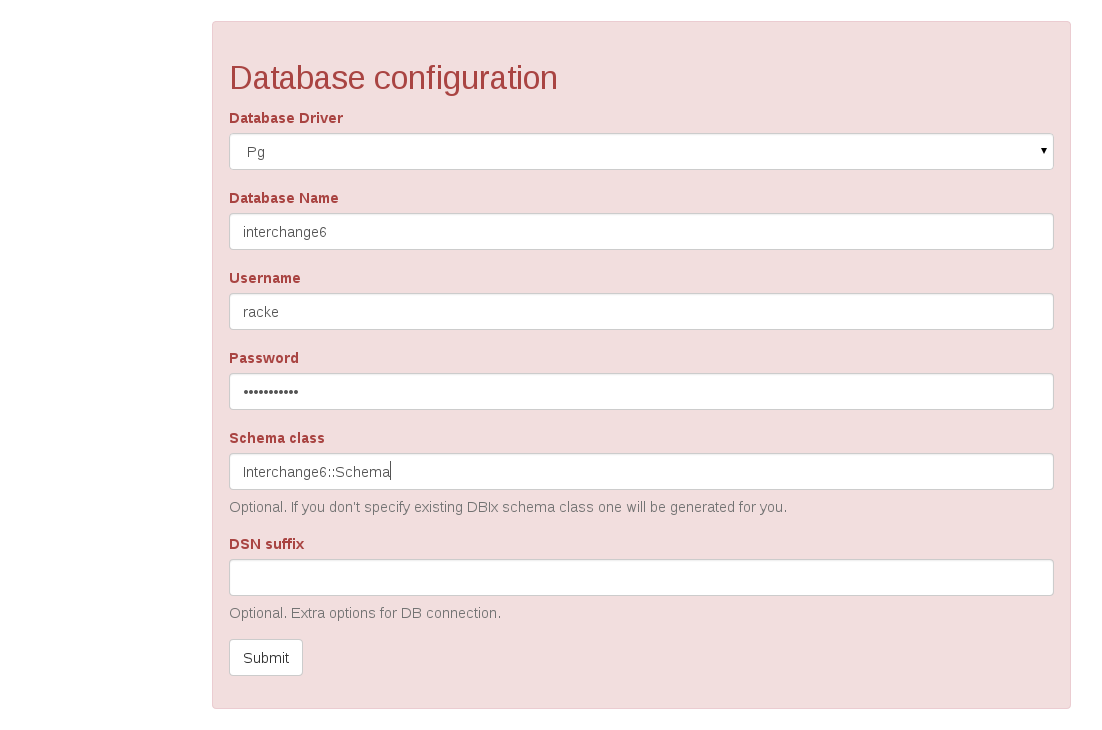
\includegraphics[width=\textwidth,height=1\textheight,keepaspectratio]{images/input.png}
  \end{center}
\end{frame}

\begin{frame}[plain]{View Products}
  \begin{center}
    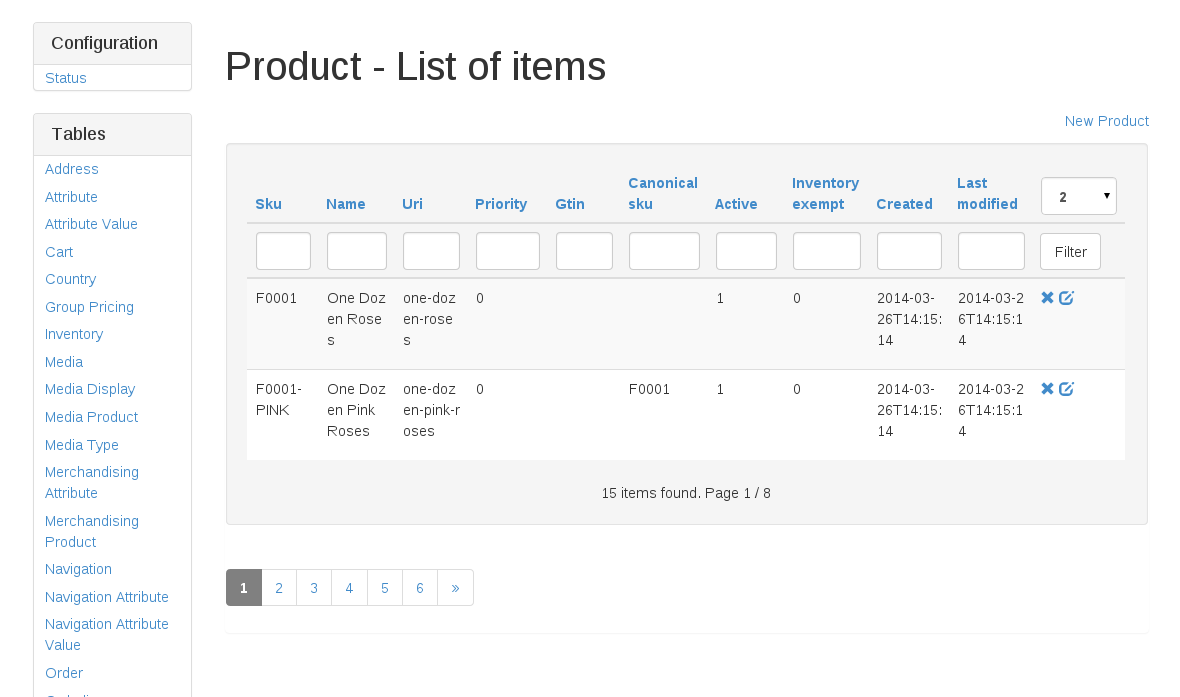
\includegraphics[width=\textwidth,height=1\textheight,keepaspectratio]{images/product.png}
  \end{center}
\end{frame}

\begin{frame}[plain]{View Product}
  \begin{center}
    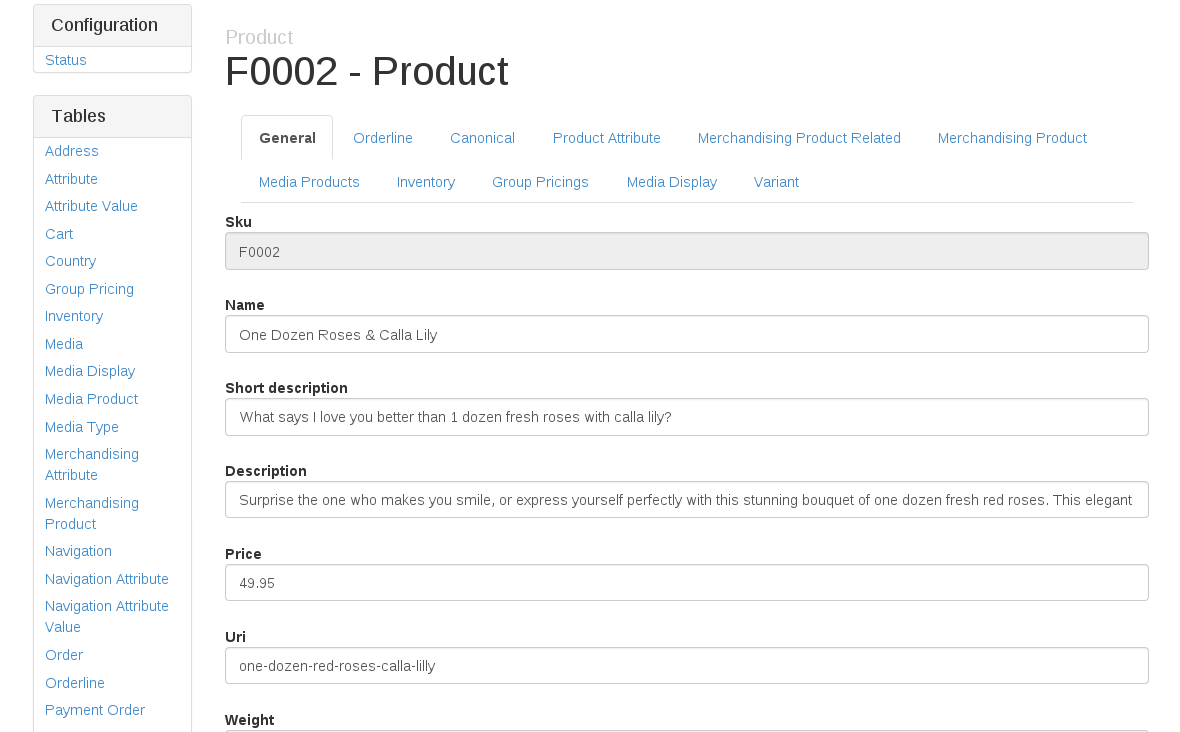
\includegraphics[width=\textwidth,height=1\textheight,keepaspectratio]{images/product-detail.png}
  \end{center}
\end{frame}

\begin{frame}[plain]{Relationship Orderline}
  \begin{center}
    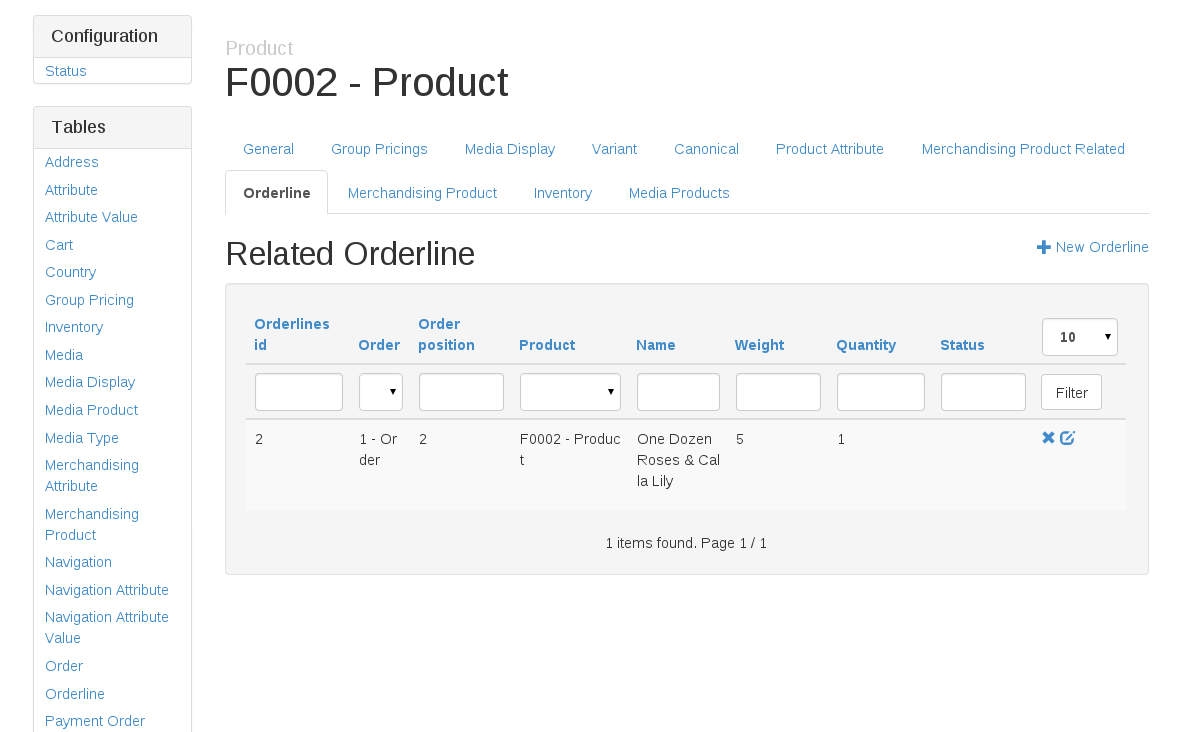
\includegraphics[width=\textwidth,height=1\textheight,keepaspectratio]{images/product-related.png}
  \end{center}
\end{frame}

\section{Dancer::Plugin::DBIC}

\begin{frame}{Overview Dancer::Plugin::DBIC}
\begin{itemize}
\item Usage
\item Configuration
\item UTF-8
\item Create schema dynamically
\end{itemize}
\end{frame}

\subsection{Usage}
\begin{frame}[fragile]{DBIx::Class without Dancer Plugin}
\begin{lstlisting}
use Interchange6::Schema;

$schema = Interchange6::Schema->connect(...);

$schema->resultset('User')->search({..});
\end{lstlisting}
\end{frame}

\begin{frame}[fragile]{DBIx::Class with Dancer Plugin}
\begin{lstlisting}
use Dancer::Plugin::DBIC;

schema->resultset('User')->search({..});

resultset('User')->search({..});

rset('User')->search({..});
\end{lstlisting}
\end{frame}

\subsection{Configuration}

Im Normalfall verwendet man nur ein Schema in seiner
Dancer-Anwendung:

\begin{frame}[fragile]{Configuration}
\begin{lstlisting}
plugins:
  DBIC:
    default:
      dsn: dbi:mysql:interchange6
      user: racke
      pass: nevairbe
      schema_class: Interchange6::Schema
\end{lstlisting}
\end{frame}

Es sind aber auch mehrere möglich:

\begin{frame}[fragile]{Multiple Schemas}
\begin{lstlisting}
plugins:
  DBIC:
    default:
      dsn: dbi:mysql:interchange6
      user: racke
      pass: nevairbe
      schema_class: Interchange6::Schema
    legacy:
      dsn: dbi:mysql:interchange5
      user: racke
      pass: nevairbe
      schema_class: Interchange5::Schema
\end{lstlisting}
\end{frame}

Das Schema \verb|legacy| wird dann wie folgt verwendet:

\begin{frame}[fragile]{Multiple Schemas}
\begin{lstlisting}
use Dancer::Plugin::DBIC;

schema('legacy')->resultset('UserDb')->search({..});
\end{lstlisting}
\end{frame}

\subsection{UTF-8}
Im Gegensatz zu Dancer::Plugin::Database bietet das DBIC-Plugin
keine automatische Unterstützung für UTF-8. Also ist die entsprechende
DBI-Option in der Konfiguration einzutragen, hier für MySQL:
\begin{frame}[fragile]{UTF-8 for MySQL}
\begin{lstlisting}
plugins:
  DBIC:
    default:
      dsn: dbi:mysql:interchange6
      user: racke
      pass: nevairbe
      schema_class: Interchange6::Schema
      options:
        mysql_enable_utf8: 1
\end{lstlisting}
\end{frame}

Die Optionen für die gängigen Datenbanken in der Übersicht:

\begin{description}
\item[SQLite] \verb|sqlite_unicode: 1|
\item[MySQL] \verb|mysql_enable_utf8: 1|
\item[PostgreSQL] \verb|pg_enable_utf8: 1| 
\end{description}

\subsection{Create schema dynamically}
Das DBIC-Plugin erzeugt dynamisch ein DBIx::Class::Schema, wenn
die Schema-Klasse (\verb|schema_class|) nicht angegeben wird.
Dazu ist das Modul DBIx::Class::Schema::Loader erforderlich.

Dies ist nicht empfehlenswert für den Produktionseinsatz, jedoch
praktisch für den TableEditor.

\begin{frame}[fragile]{Create schema dynamically}
\begin{itemize}
\item \verb|schema_class| missing in configuration
\item DBIx::Class::Schema::Loader
\item test and development
\item TableEditor
\end{itemize}
\end{frame}

\section{Dancer::Session::DBIC}

\begin{frame}<handout:0>{Overview Dancer::Session::DBIC}
\begin{itemize}
\item engines
\item configuration
\item serialization
\item session expiration
\end{itemize}
\end{frame}

\subsection{Engines}
\begin{frame}{Engines}
\begin{itemize}
\item Templates \\
TT, Xslate, Flute, ...
\item Sessions \\ 
Storable, Database, DBIC
\item Logger \\
File, Syslog
\item Serializer  \\
JSON, YAML, XML
\end{itemize}
\end{frame}

Die Sessionengines werden in Dancer für gewöhnlich transparent
für den Anwendungscode in der Konfiguration eingerichtet:

\begin{frame}{Configuration}
\begin{description}
\item[session] name of session engine (DBIC)
\item[session\_options] options
\item[session\_expires] expiration date
\end{description}
\end{frame}

Das ermöglicht es, auf dem Liveserver eine effizientere Engine
zu verwenden (z.B. Storable) und auf dem Entwicklungsserver
eine Engine, die einem beim debuggen hilft (z.B. YAML).

Die Optionen für Dancer::Session::DBIC ähneln der Konfiguration von
Dancer::Plugin::DBIC, zusätzlich können wir festlegen wie
die Sessions aus der Datenbank abgerufen werden können:

\begin{description}
\item[resultset] DBIx::Class resultset
\item[id\_column] primary key
\item[data\_column] field for session data 
\end{description}

Das sieht dann z.B. für \href{https://metacpan.org/pod/Interchange6::Schema}{Interchange6::Schema} (Version 0.015) so aus:

\begin{frame}[fragile]{Configuration}
\begin{lstlisting}
session: "DBIC"
session_options:
  dsn: dbi:mysql:interchange6
  user: racke
  pass: nevairbe
  schema_class: Interchange6::Schema
  resultset: Session
  id_column: sessions_id
  data_column: session_data
session_expires: 12 hours
\end{lstlisting}
\end{frame}

Die Konfiguration kann aber ebenso im Hauptmodul
stattfinden:

\begin{frame}[fragile]{Configuration}
\begin{lstlisting}
set session => 'DBIC';
set session_options => {schema => schema};
\end{lstlisting}
\end{frame}

\subsection{Example table}

Folgendermaßen sieht die Tabelle \verb|sessions| aus,
die vom Schema \href{https://metacpan.org/pod/Interchange6::Schema}{Interchange6::Schema} (Version 0.015)
erzeugt wird:

\begin{frame}[fragile]{Example table}
\begin{lstlisting}
CREATE TABLE `sessions` (
  `sessions_id` varchar(255) NOT NULL,
  `session_data` text NOT NULL,
  `created` datetime NOT NULL,
  `last_modified` datetime NOT NULL,
  PRIMARY KEY (`sessions_id`)
) ENGINE=InnoDB;
\end{lstlisting}
\end{frame}

\subsection{Serializer}
\begin{frame}[fragile]{Serializer}
\begin{lstlisting}
set 'session_options' => {
    schema       => schema,
    serializer   => sub { YAML::Dump(@_); },
    deserializer => sub { YAML::Load(@_); },
};
\end{lstlisting}
\end{frame}

\subsection{Session expiration}

Beim Überschreiten der erlaubten Ablaufzeit wird die Sitzung
ungültig, sie wird jedoch nicht in der Datenbank gelöscht.
Dafür ist ein Skript zur regelmäßigen Löschung der
abgelaufenen Datensätze erforderlich.

JSON
andere DBIC connection?
tests?

\begin{frame}[fragile]{Session expiration}
\begin{itemize}
\item remove old sessions from database
\item \verb|Interchange6::Schema::Resultset::Session|
\end{itemize}
\begin{lstlisting}
$schema->resultset('Session')->expire('12 hours');
\end{lstlisting}
\end{frame}

\section{TableEditor}

\begin{frame}<handout:0>{Overview TableEditor}
\begin{itemize}
\item Installation
\item Frontend
\item Routes
\item Login
\item Relationships
% \item Limitations
\item Configuration
\end{itemize}
\end{frame}

\subsection{Installation}
Im günstigsten Fall kann die Installation mit 4 Schritten
erledigt werden:

\begin{frame}[fragile]{Installation}
\begin{lstlisting}
git clone https://github.com/interchange/TableEditor
cd TableEditor
cpanm .
./bin/app.pl
\end{lstlisting}
\end{frame}

\begin{frame}[fragile]{Driver}
\begin{itemize}
\item DBD::mysql
\item DBD::Pg
\item ...
\end{itemize}
\end{frame}

\subsection{Frontend}
Das Frontend für den TableEditor ist mit Angular und Bootstrap erstellt.
Das Theme kann sehr einfach durch Austausch der CSS-Datei für Bootstrap
geändert werden.

\begin{frame}<handout:0>{Frontend}
\begin{itemize}
\item Angular
\begin{itemize}
\item Routes for the frontend
\item XHR requests to REST API
\item JSON
\end{itemize}
\item Bootstrap
\item Theme
\end{itemize}
\end{frame}

\subsection{Routes}
\begin{frame}[fragile]{Routes}
\begin{lstlisting}
get '/:class/:id' => require_login sub {
    # retrieve database record and add relationships
    ...

    return to_json($data, {allow_unknown => 1});
};
\end{lstlisting}
\end{frame}

\subsection{Login}

Für die Integration von Authentifizierung in eine Dancer-Anwendung empfehlen
wir wärmestens das
\href{https://metacpan.org/pod/Dancer::Plugin::Auth::Extensible}{Auth::Extensible}
Plugin.

\begin{frame}{Login}
\begin{itemize}
\item Dancer::Plugin::Auth::Extensible
\item Provider
\begin{itemize}
\item Unix
\item DBIC
\end{itemize}
\item Database \textit{(planned)}
\end{itemize}
\end{frame}

\subsection{Relationships}

Beziehungen werden automatisch angezeigt.

\begin{frame}{Relationships}
\begin{itemize}
\item belongs\_to
\item has\_many
\item might\_have
\item has\_one
\item many\_to\_many \\
      needs to be configured
\end{itemize}
\end{frame}

Filter

Es fehlen Felder in related orderline (Übersicht)

Different DBIC keys

Paging

% \subsection{Limitations}
% \begin{frame}{Limitations}
% \begin{itemize}
% \item Primary key for \textbf{one} column only
% \item Speed (complex schemas)
% \item Error handling
% \end{itemize}
% \end{frame}

\subsection{Configuration}
\begin{frame}[fragile]{Configuration}
\begin{itemize}
\item Auth::Extensible
\item DBIC
\begin{itemize}
\item \verb|default|
\end{itemize}
\end{itemize}
\end{frame}

\begin{frame}{Planned Features}
\begin{itemize}
\item Search (Solr)
\item Select schema
\item Debian packages
\end{itemize}
\end{frame}


\section{Forecast and Contribution}

\subsection{Development}

Das Git-Repository für den TableEditor befindet sich auf Github:

\begin{frame}{Development}
\url{https://github.com/interchange/TableEditor}
\end{frame}

\subsection{Dancer2}

Was ist mit Dancer2 ?

Für Dancer2 existiert bereits ein Plugin:

\url{https://metacpan.org/pod/Dancer2::Plugin::DBIC}

Die Sessionengine und der TableEditor wurden noch nicht auf Dancer2 portiert.

\begin{frame}{Dancer2}
  \begin{description}
  \item[Plugin::DBIC] \url{https://metacpan.org/pod/Dancer2::Plugin::DBIC}
  \item[Session::DBIC] \url{https://metacpan.org/pod/Dancer2::Session::DBIC}
  \item[TableEditor] not yet ported
  \end{description}
\end{frame}

% \section{Testing}
% DBIC, Plugin
% Testdatabase

\subsection{Further reading}

\url{https://github.com/castaway/dbix-class-book}

\subsection{Slides}

\begin{frame}{Slides}
Slides:
\url{http://www.linuxia.de/talks/czpw2014/dancer-dbic-en-beamer.pdf}
\end{frame}

\end{document}

%%% Local Variables: 
%%% mode: latex
%%% TeX-master: t
%%% End: 
